% Copyright (C) 2010,2011,2012,2013,2014,2015,2016 The ESPResSo project
% Copyright (C) 2002,2003,2004,2005,2006,2007,2008,2009,2010 
%    Max-Planck-Institute for Polymer Research, Theory Group
%  
% This file is part of ESPResSo.
%   
% ESPResSo is free software: you can redistribute it and/or modify it
% under the terms of the GNU General Public License as published by the
% Free Software Foundation, either version 3 of the License, or (at your
% option) any later version.
%  
% ESPResSo is distributed in the hope that it will be useful, but
% WITHOUT ANY WARRANTY; without even the implied warranty of
% MERCHANTABILITY or FITNESS FOR A PARTICULAR PURPOSE.  See the GNU
% General Public License for more details.
%  
% You should have received a copy of the GNU General Public License
% along with this program.  If not, see <http://www.gnu.org/licenses/>.
%
\chapter{Analysis in Tcl}
\label{chap:analysis}
\index{analysis}
\newescommand{analyze}

\todo{Add a comment to the UG that the analysis routines in \es{} with
  Python currently require the user to `from espressomd import
  analyze.'}

\es has two fundamentally different classes of observables for
analyzing the systems.  On the one hand, some observables are
computed from the Tcl level. In that case, the observable is measured
in the moment that the corresponding Tcl function is called, and the
results are returned to the Tcl script. In general, observables in
this class should only be computed after a large number of timesteps,
as switching forth and back between the C- and the Tcl-level is
costly. This chapter describes all observables in this class.

On the other hand, some observables are computed and stored in the
C-core of \es during a call to the function \keyword{integrate}, while
they are set up and their results are collected from the Tcl level.
These observables are more complex to implement and offer less
flexibility, while the are significantly faster and more memory
efficient, and they can be set up to be computed every few
timesteps. The observables in this class are described in chapter
\ref{chap:analysis-core}.

The class of Tcl-level analysis functions is mainly controlled via the
\keyword{analyze} command. It has two main uses: Calculation of
observables (\keyword{analyze \var{observable}}) and definition and
analysis of topologies in the system (\keyword{analyze \var{topology
    command}}).  In addition, \es offers the command \keyword{uwerr}
(see section \ref{sec:uwerr} for computing statistical errors in time
series.

\section{Available observables}

The command \keyword{analyze} provides online-calculation of local and
global observables. 

\subsection{Minimal distances between particles}
\label{analyze:mindist}
\label{analyze:distto}
\analyzeindex{minimal particle distance}
\analyzeindex{particle distance}

\begin{essyntax}
  \variant{1} analyze mindist \opt{\var{type\_list\_a} \var{type\_list\_b}}
  \variant{2} analyze distto \var{pid}
  \variant{3} analyze distto \var{x} \var{y} \var{z}
\end{essyntax}

Variant \variant{1} returns the minimal distance between two particles
in the system. If the type-lists are given, then the minimal distance
between particles of only those types is determined.

\keyword{distto} returns the minimal distance of all particles to
particle \var{pid} (variant \variant{2}), or to the coordinates
(\var{x}, \var{y}, \var{z}) (Variant \variant{3}).

\subsection{Particles in the neighbourhood}
\label{analyze:nbhood}
\analyzeindex{particles in the neighbourhood}

\begin{essyntax}
 \variant{1} analyze nbhood \var{pid} \var{r\_catch}
 \variant{2} analyze nbhood \var{x} \var{y} \var{z}
 \var{r_catch}
\end{essyntax}
Returns a Tcl-list of the particle ids of all particles within a given
radius \var{r\_catch} around the position of the particle with number
\var{pid} in variant \variant{1} or around the spatial coordinate
(\var{x}, \var{y}, \var{z}) in variant \variant{2}.

\subsection{Particle distribution}
\label{analyze:distribution}
\analyzeindex{particle distribution}

\begin{pysyntax}
  \object{
    espressomd.analyze.Analysis(system)
  }{
    distribution
  }{
    system = \arg{system},
    type_list_a = \arg{list of ints},
    type_list_b = \arg{list of ints},
    r_min = \arg{float},
    r_max = \arg{float},
    r_bins = \arg{int},
    log_flag = \arg{int},
    int_flag = \arg{int}
  }
\end{pysyntax}

\begin{essyntax}
  analyze distribution \var{part\_type\_list\_a} \var{part\_type\_list\_b}
  \opt{\var{rmin} \opt{\var{rmax} \opt{\var{rbins} 
        \opt{\var{log\_flag} \opt{\var{int\_flag}}}}}}
\end{essyntax}
Returns its parameters and the distance distribution of particles 
(probability of finding a particle of type \var{a} at a certain distance 
around a particle of type \var{b}, disregarding the fact that a spherical 
shell of a larger radius covers a larger volume) with
types specified in \var{part\_type\_list\_a} around particles with
types specified in \var{part\_type\_list\_b} with distances between
\var{rmin} and \var{rmax}, binned into \var{rbins} bins. The
bins are either equidistant (if $\var{log\_flag} = 0$) or
logarithmically equidistant (if $\var{log\_flag} \geq 1$). If an
integrated distribution is required, use $\var{int\_flag}=1$. The
distance is defined as the \emph{minimal} distance between a particle
of one group to any of the other group.

\minisec{Output format} 

The output corresponds to the blockfile format (see section
\vref{sec:structured-file-format}):
\begin{code}
\{ \var{parameters} \} 
\{ 
  \{ \var{r} \var{dist(r)} \} 
  \vdots 
\}
\end{code}

\subsection{Radial density map}
\label{analyze:radialdensitymap}

\begin{essyntax}
  analyze radial_density_map \var{xbins} \var{ybins} \var{xrange} \var{yrange}
  \opt{\var{axisofrotation} \var{centerofrotation} \var{beadtypelist}
  \opt{\var{thetabins}}}
\end{essyntax}

Returns the radial density of particles around a given
axis. Parameters are:
\begin{itemize}
\item \var{xbins} histogram bins in x direction.
\item \var{ybins} histogram bins in y direction.
\item \var{xrange} range for analysis in x direction.
\item \var{yrange} range for analysis in y direction.
\item \var{axisofrotation} rotate around given axis. (x, y, or z)
\item \var{centerofrotation} rotate around given point.
\item \var{beadtypelist} only analyze beads of given types.
\item \var{thetabins} histogram bins in angle theta.
\end{itemize}

\minisec{Caveat}

This command does not do what you might expect.  Here is an overview
of the currently identified properties.
\begin{enumerate}
\item \var{xbins} is the number of bins along the axis of rotation.
\item \var{ybins} is the number of bins in the radial direction.
\item The centre point (\var{centerofrotation}) of the cylinder is
  located in the lower cap, i.e., \var{xrange} is the height of the
  cylinder with respect to this centre point.
\item The bins are distributed along \var{axisofrotation} starting
  from 0 (\var{centerofrotation}).
\item The \var{thetabins} seem to average with respect to the centre
  of mass of the particles in the individual bins rather than with
  respect to the central axis, which one would think is natural.
\end{enumerate}

\subsection{Cylindrical Average}
\label{analyze:cylindricalaverage}

\begin{pysyntax}
  \object{
    espressomd.analyze.Analysis(system)
  }{
    cylindrical_average
  }{
    system = \arg{system},
    center = \arg{3 floats},
    direction = \arg{3 floats},
    length = \arg{float},
    radius = \arg{float},
    bins_axial = \arg{int},
    bins_radial = \arg{int},
    types = \arg{list of ints}
  }
\end{pysyntax}

\begin{essyntax}
  analyze cylindrical_average \var{center} \var{direction}
  \var{length} \var{radius} \var{bins\_axial} \var{bins\_radial}
  \opt{\var{types}}
\end{essyntax}

The command returns a list of lists.  The outer list contains all data
combined whereas each inner list contains one line.  Each lines stores
a different combination of the radial and axial index.  The output
might look something like this
\begin{verbatim}
{ { 0 0 0.05 -0.25 0.0314159 0 0 0 0 0 0 }
  { 0 1 0.05 0.25 0.0314159 31.831 1.41421 1 0 0 0 }
  ... }
\end{verbatim}
In this case two different particle types were present.  The columns
of the respective lines are coded like this
\begin{SaveVerbatim}{output}
index_radial index_axial pos_radial pos_axial binvolume density v_radial v_axial density v_radial v_axial
0            0           0.05       -0.25     0.0314159 0       0        0       0       0        0
0            1           0.05       0.25      0.0314159 31.831  1.41421  1       0       0        0
\end{SaveVerbatim}
\bigbreak\noindent%
\resizebox{\linewidth}{!}{\BUseVerbatim{output}}
\bigbreak\noindent%
%
As one can see the columns \keyword{density}, \keyword{v_radial}, and
\keyword{v_axial} appear twice.  The order of appearance corresponds
two the order of the types in the argument \var{types}.  For example
if \var{types} was set to \Verb|{0 1}| then the first triple is
associated to type 0 and the second triple to type 1.

After knowing what the output looks like we might want to have more
information on how to input data.
\begin{itemize}
\item \var{center} is a double list containing the coordinates of the
  centre point of the cylinder.
\item \var{direction} is a double list containing a (not necessarily
  normalised) vector.
\item \var{length} is the total length of the cylinder.
\item \var{radius} is the radius of the cylinder.
\item \var{bins\_axial} is the number of bins along the \var{direction}
  vector.
\item \var{bins\_radial} is the number of bins in radial direction.
\item \var{types} is an int list of the type IDs.
\end{itemize}
Because all of this text is super abstract we additionally drew a
picture of what these variables actually mean, see
figure~\ref{fig:cylindricalaverage}.

\begin{figure}[tb]
  \centering
  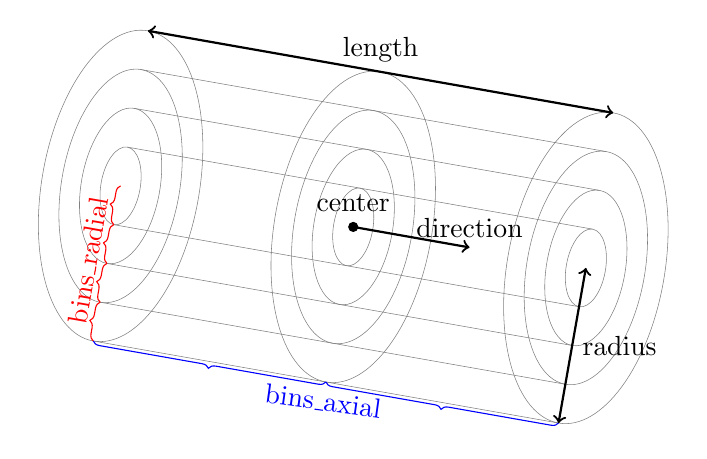
\begin{tikzpicture}[dot/.style={draw,fill,circle,inner sep=1pt},rotate=-100]
    \pgfmathsetmacro\H{3}
    \foreach \r in { .5, 1, 1.5, 2 } {
      \foreach \h in { -\H, 0, \H }
        \draw[help lines] (0,\h) ellipse ({\r} and {.5*\r});
      \draw[help lines] (-\r,-\H) -- (-\r,\H);
      \draw[help lines] (+\r,-\H) -- (+\r,\H);
    }
    \draw[thick,->] (0,0) node[dot,label={above:center}] {} -- (0,1.5) node[above] {direction};
    \foreach \h in { 0, \H }
      \draw[blue,decoration=brace,decorate] (2,\h) -- (2,\h-\H);
    \path (2,-\H) -- node[blue,below,rotate=-8] {bins\_axial} (2,\H);
    \foreach \r in { .5, 1, 1.5, 2 }
      \draw[red,decoration=brace,decorate] (\r,-\H) -- (\r-.5,-\H);
    \path (2,-\H) -- node[red,above,rotate=80] {bins\_radial} (0,-\H);
  
    \draw[thick,<->] (0,\H) -- node[right] {radius} (2,\H);
    \draw[thick,<->] (-2,-\H) -- node[above] {length} (-2,\H);
  \end{tikzpicture}
  \caption{Illustration of the parameters for the \keyword{analyze
      cylindrical_average} command.}
  \label{fig:cylindricalaverage}
\end{figure}


\subsection{Modes}
\label{analyze:modes2d}

\begin{essyntax}
  analyze modes2d
\end{essyntax}

Analyzes the modes of a configuration. Requires that a grid is set and
that the system contains more than two particles. Output are four
numbers in the order:

\begin{displaymath}
ht_{RE}\qquad ht_{IM}\qquad \theta_{RE}\qquad \theta_{IM}
\end{displaymath}

\subsection{Lipid orientation}
\label{analyze:lipids}

\begin{essyntax}
  \variant{1} analyze get_lipid_orients
  \variant{2} analyze lipid_orient_order
\end{essyntax}

\todo{Document the usage!}

\subsection{Bilayers}
\label{analyze:bilayers}

\begin{essyntax}
  \variant{1} analyze bilayer_set
  \variant{2} analyze bilayer_density_profile
\end{essyntax}

\todo{Document the usage!}

\subsection{GPB}
\label{analyze:cellgpb}

\begin{essyntax}
  analyze cell_gpb \var{Manning parameter} \var{outer cell radius}
  \var{inner cell radius} \opt{\var{accuracy}
    \opt{\var{number of interactions}}}
\end{essyntax}

\todo{Document the usage and what it is!}

\subsection{Get folded positions}
\label{analyze:folded}

\begin{essyntax}
  analyze get_folded_positions \opt{-molecule} \opt{shift \var{x} \var{y} \var{z}}
\end{essyntax}

Outputs the folded positions of particles. Without any parameters, the
positions of all particles are given, folded to the box length. The
optional parameter \keyword{-molecule} ensures that molecules
(particle groups) are kept intact. The optional shift parameters can
be used to shift the not separated molecules if needed.

\subsection{Vkappa}
\label{analyze:Vkappa}

\begin{pysyntax}
  \object{
    espressomd.analyze.Analysis(system)
  }{
    Vkappa
  }{
    system = \arg{system},
    mode = \arg{string},
    Vk1 = \arg{float},
    Vk2 = \arg{float},
    avk = \arg{float}
  }
\end{pysyntax}
\begin{essyntax}
  analyze Vkappa \opt{\alt{ reset \asep read \asep set \var{V_{\kappa, 1}} \var{V_{\kappa, 2}} \var{avk} } }
\end{essyntax}

Calculates the compressibility $V \times \kappa_T$ through the Volume fluctuations
$V \times \kappa_T = \beta \left(\langle V^2\rangle - \langle V \rangle^2\right)$ \cite{kolb99a}.
Given no arguments this function calculates and returns the current value of the
running average for the volume fluctuations.  
The argument \keyword{reset} clears the currently stored values. With \keyword{read}
the cumulative mean volume, cumulative mean squared volume and how many samples were
used can be retrieved. Likewise the option \keyword{set} enables you to set those. 

\subsection{Radial distribution function}
\label{analyze:rdf}
\label{analyze:<rdf>}
\analyzeindex{radial distribution function $g(r)$}

\begin{pysyntax}
  \object{
    espressomd.analyze.Analysis(system)
  }{
    rdf
  }{
    system = \arg{system},
    rdf_type = \arg{string},
    type_list_a = \arg{list of ints},
    type_list_b = \arg{list of ints},
    r_min = \arg{float (0.0)},
    r_max = \arg{float},
    r_bins = \arg{int (100)}
    n_conf = \arg{int}
  }
\end{pysyntax}

\begin{essyntax}
  analyze \alt{rdf \asep <rdf>} 
  \var{part\_type\_list\_a} \var{part\_type\_list\_b} 
  \opt{\var{rmin} \var{rmax} \var{rbins}}
\end{essyntax}
Returns its parameters and the radial distribution function (rdf) of
particles with types specified in \var{part\_type\_list\_a} around
particles with types specified in \var{part\_type\_list\_b}. The range
is given by \var{rmin} and \var{rmax} and is divided into
\var{rbins} equidistant bins.

\minisec{Output format}

The output corresponds to the blockfile format (see section
\vref{sec:structured-file-format}):
\begin{code}
\{ \var{parameters} \} 
\{ 
  \{ \var{r} \var{rdf(r)} \} 
  \vdots
\}
\end{code}

\subsection{Structure factor}
\label{analyze:structurefactor}
\analyzeindex{structure factor $S(q)$}

\begin{pysyntax}
  \object{
    espressomd.analyze.Analysis(system)
  }{
    structure_factor
  }{
    system = \arg{system},
    sf_types = \arg{list of ints},
    sf_order = \arg{int}
  }
\end{pysyntax}

\begin{essyntax}
  analyze structurefactor \var{types} \var{order}
\end{essyntax}

Returns the spherically averaged structure factor $S(q)$ of particles
specified in \var{types}. $S(q)$ is calculated for all possible
wave vectors, $\frac{2\pi}{L} <= q <= \frac{2\pi}{L}\var{order}$. Do
not choose parameter \var{order} too large, because the number of
calculations grows as $\var{order}^3$. 


\minisec{Output format} 

The output corresponds to the blockfile format (see section
\vref{sec:structured-file-format}):
\begin{code}
\{ \var{q\_value} \var{S(q)\_value} \} 
\vdots
\end{code}

\subsection{Van-Hove autocorrelation function $G(r,t)$}
\label{analyze:vanhove}
\analyzeindex{van Hove autocorrelation function $G(r,t)$}
\begin{essyntax}
  analyze vanhove \var{type} \var{rmin} \var{rmax} \var{rbins}
  \opt{\var{tmax}}
\end{essyntax}
Returns the van Hove auto correlation function $G(r,t)$ and the mean
square displacement $msd(t)$ for particles of type \var{ptype} for the
configurations stored in the array configs. This tool assumes that the
configurations stored with \codebox{analyze append} (see section
\vref{sec:stored-configs}) are stored at equidistant time intervals.
$G(r,t)$ is calculated for each multiple of this time intervals. For
each time t the distribution of particle displacements is calculated
according to the specification given by \var{rmin}, \var{rmax} and
\var{rbins}. Optional argument \var{tmax} defines the maximum value
of $t$ for which $G(r,t)$ is calculated. If it is omitted or set to
zero, maximum possible value is used.
If the particles perform a random walk (\ie a normal
diffusion process) $G(r,t)/r^2$ is a Gaussian distribution for all
times.  Deviations of this behavior hint on another diffusion process
or on the fact that your system has not reached the diffusive regime.
In this case it is also very questionable to calculate a diffusion
constant from the mean square displacement via the Stokes-Einstein
relation. 

\minisec{Output format}
The output corresponds to the blockfile format (see section
\vref{sec:structured-file-format}):
\begin{code}
\{ msd \{ \var{msd(0)} \var{msd(1)} \dots \} \} 
\{ vanhove \{ \{ \var{G(0,0)} \var{G(1,0)} \dots \} 
            \{ \var{G(0,1)} \var{G(1,1)} \dots \}
\vdots
          \}
\}
\end{code}

The $G(r,t)$ are normalized such that the integral over space always
yields $1$.

\subsection{Center of mass}
\label{analyze:centermass}
\analyzeindex{center of mass}
\begin{essyntax}
  analyze centermass \var{part\_type}
\end{essyntax}
Returns the center of mass of particles of the given type.

\subsection{Moment of inertia matrix}
\label{analyze:momentofinteratiamatrix}
\label{analyze:find-principal-axis}
\analyzeindex{moment of inertia matrix}
\analyzeindex{principal axis of the moment of inertia}

\begin{pysyntax}
  \object{
    espressomd.analyze.Analysis(system)
  }{
    momentofinertiamatrix
  }{
    system = \arg{system},
    p_type = \arg{int}
  }
\end{pysyntax}
\begin{essyntax}
  \variant{1} analyze momentofinertiamatrix { \var{typeid} } 
  \variant{2} analyze find_principal_axis \var{typeid}
\end{essyntax}
Variant \variant{1} returns the moment of inertia matrix for particles
of given type \var{typeid}. The output is a list of all the elements
of the 3x3 matrix. Variant \variant{2} returns the eigenvalues and
eigenvectors of the matrix.

\subsection{Gyration tensor}
\label{analyze:gyration-tensor}
\analyzeindex{gyration tensor}

\begin{pysyntax}
  \object{
    espressomd.analyze.Analysis(system)
  }{
    gyration_tensor
  }{
    system = \arg{system},
    p_type = \arg{int}
  }
\end{pysyntax}
\begin{essyntax}
  analyze gyration\_tensor \opt{\var{typeid}} 
\end{essyntax}
Analyze the gyration tensor of particles of a given type \var{typeid},
or of all particles in the system if no type is given.
Returns a Tcl-list containing the squared radius of gyration,
 three shape descriptors (asphericity, acylindricity,
 and relative shape anisotropy), eigenvalues of the gyration tensor and their
corresponding eigenvectors. The eigenvalues are sorted in descending order.

\subsection{Aggregation}
\label{analyze:aggregation}
\analyzeindex{aggregation}

\begin{essyntax}
  analyze aggregation \var{dist\_criteria} \var{s\_mol\_id}
  \var{f\_mol\_id} \opt{\var{min\_contact} \opt{\var{charge\_criteria}}}
\end{essyntax}
Returns the aggregate size distribution for the molecules in the
molecule id range \var{s\_mol\_id} to \var{f\_mol\_id}. If any
monomers in two different molecules are closer than
\var{dist\_criteria} they are considered to be in the same aggregate.
One can use the optional \var{min\_contact} parameter to specify a
minimum number of contacts such that only molecules having at least
\var{min\_contact} contacts will be considered to be in the same
aggregate. The second optional parameter \var{charge\_criteria}
enables one to consider aggregation state of only oppositely charged
particles.

\subsection{Identifying pearl-necklace structures}
\label{analyze:necklace}
\analyzeindex{pearl-necklace structures}

\begin{essyntax}
 analyze necklace \var{pearl\_threshold} \var{back\_dist} \var{space\_dist}
\var{first} \var{length} 
\end{essyntax}
Algorithm for identifying pearl necklace structures for
polyelectrolytes in poor solvent \citep{limbach03a}. The first three
parameters are tuning parameters for the algorithm:
\var{pearl\_threshold} is the minimal number of monomers in a pearl.
\var{back\_dist} is the number of monomers along the chain backbone
which are excluded from the space distance criterion to form clusters.
\var{space\_dist} is the distance between two monomers up to which
they are considered to belong to the same clusters. The three
parameters may be connected by scaling arguments. Make sure that your
results are only weakly dependent on the exact choice of your
parameters. For the algorithm the coordinates stored in partCfg are
used. The chain itself is defined by the identity first of its first
monomer and the chain length length.  Attention: This function is very
specific to the problem and might not give useful results for other
cases with similar structures.

\subsection{Finding holes}
\label{analyze:holes}
\analyzeindex{finding holes}

\begin{essyntax}
  analyze holes \var{typeid_\mathrm{probe}} \var{mesh\_size}
  \begin{features}
    \required{LENNARD_JONES}
  \end{features}
\end{essyntax}
Function for the calculation of the unoccupied volume (often also
called free volume) in a system. Details can be found in
\citet{schmitz00a}.  It identifies free space in the simulation box
via a mesh based cluster algorithm.  Free space is defined via a probe
particle and its interactions with other particles which have to be
defined through LJ interactions with the other existing particle types
via the inter command before calling this routine. A point of the mesh
is counted as free space if the distance of the point is larger than
LJ_cut+LJ_offset to any particle as defined by the LJ interaction
parameters between the probe particle type and other particle types.\
How to use this function:\ Define interactions between all (or the
ones you are interested in) particle types in your system and a
fictitious particle type.  Practically one uses the van der Waals radius
of the particles plus the size of the probe you want to use as the
Lennard Jones cutoff. The mesh spacing is the box length divided by
the \var{mesh_size}.

\minisec{Output format}
\begin{code}
\{ \var{n\_holes} \var{mean\_hole\_size} \var{max\_hole\_size} \var{free\_volume\_fraction} 
    \{ \var{sizes} \}
    \{ \var{surfaces} \} 
    \{ \var{element\_lists} \} 
\} 
\end{code}

A hole is defined as a continuous cluster of mesh elements that belong
to the unoccupied volume. Since the function is quite rudimentary it
gives back the whole information suitable for further processing on
the script level. \var{sizes} and \var{surfaces} are given in number
of mesh points, which means you have to calculate the actual size via
the corresponding volume or surface elements yourself. The complete
information is given in the element_lists for each hole. The element
numbers give the position of a mesh point in the linear representation
of the 3D grid (coordinates are in the order x, y, z). Attention: the
algorithm assumes a cubic box. Surface results have not been tested.
\todo{I think there is still a bug in there (Hanjo)}.


\subsection{Temperature of the LB fluid}
\label{analyze:lbtemp}
\analyzeindex{fluid temperature}

\begin{essyntax}
  \require{1 or 2 or 3}{analyze fluid temp}
  \begin{features}
  \required[1]{LB}
  \required[2]{LB_GPU}
  \required[3]{ELECTROKINETICS}
  \end{features}
\end{essyntax}

This command returns the temperature of the lattice-Boltzmann (LB)
fluid, see Chapter~\ref{sec:lb}, by averaging over the fluid nodes. In
case \feature{LB_BOUNDARIES} or \feature{LB_BOUNDARIES_GPU} are
compiled in and boundaries are defined, only the available fluid
volume is taken into account.

\subsection{Momentum of the System}
\label{analyze:momentum}
\analyzeindex{system momentum}
\begin{pysyntax}
  \object{
    espressomd.analyze.Analysis(system)
  }{
    calc_re
  }{
    system = \arg{system},
    include_particles = \arg{bool},
    include_lbfluid = \arg{bool},
  }
\end{pysyntax}
\begin{essyntax}
    analyze momentum \opt{\alt{particles \asep lbfluid}}
\end{essyntax}
This command returns the total linear momentum of the particles and the lattice-Boltzmann (LB) fluid, if one exists. Giving the optional parameters either
causes the command to ignore the contribution of LB or of the particles.

\subsection{Energies}
\label{analyze:energy}
\analyzeindex{energies}

\begin{essyntax}
  \variant{1} analyze energy
  \variant{2} analyze energy \alt{total \asep kinetic \asep coulomb \asep magnetic}
  \variant{3} analyze energy bonded \var{bondid}
  \variant{4} analyze energy nonbonded \var{typeid1} \var{typeid2}
\end{essyntax}
\todo{Describe the different energies components returned by the
  different commands!}
Returns the energies of the system. Variant \variant{1} returns all
the contributions to the total energy. Variant \variant{2} returns the
numerical value of the total energy or its kinetic or Coulomb or magnetic
contributions only. Variants \variant{3} and \variant{4} return the
energy contributions of the bonded resp. non-bonded interactions.

\minisec{Output format (variant \variant{1})}
\begin{code}
\{ energy \var{value} \} \{ kinetic \var{value} \} \{ interaction \var{value} \} \dots 
\end{code}

\subsection{Pressure}
\label{analyze:pressure}
\analyzeindex{pressure}

\begin{essyntax}
  \variant{1} analyze pressure
  \variant{2} analyze pressure total
  \variant{3} analyze pressure \alt{totals \asep ideal \asep coulomb
    \asep \\tot_nonbonded_inter \asep tot_nonbonded_intra \asep vs_relative}
  \variant{4} analyze pressure bonded \var{bondid}
  \variant{5} analyze pressure nonbonded \var{typeid1} \var{typeid2}
  \variant{6} analyze pressure nonbonded_intra \opt{\var{typeid}}
  \variant{7} analyze pressure nonbonded_inter \opt{\var{typeid}}
\end{essyntax}

Computes the pressure and its contributions in the system. Variant
\variant{1} returns all the contributions to the total pressure.
Variant \variant{2} will return the total pressure only.  Variants
\variant{3}, \variant{4} and \variant{5} return the corresponding
contributions to the total pressure.

\warning{Pressure works only with certain interactions and
features. Read in detail before use!}

\todo{Document arguments nb_inter, nb_intra, tot_nb_inter and
  tot_nb_intra}

The pressure is calculated (if there are no electrostatic interactions) by 
\begin{equation}
\label{eq:ptens}
  p = \frac{2E_{kinetic}}{Vf} + \frac{\sum_{j>i} {F_{ij}r_{ij}}}{3V}
\end{equation}
where $f=3$ is the number of translational degrees of freedom of each particle, $V$
is the volume of the system, $E_{kinetic}$ is the kinetic energy, $F_{ij}$ the force between
particles i and j, and $r_{ij}$ is the distance between them.  The kinetic energy divided by the
degrees of freedom is
\begin{equation}
\frac{2E_{kinetic}}{f} = \frac{1}{3}\sum_{i} {m_{i}v_{i}^{2}}.
\end {equation}

Note that Equation~\ref{eq:ptens} can only be applied to pair potentials and central forces.
Description of how contributions from other interactions are calculated is beyond the scope
of this manual. Three body potentials are implemented following the procedure in 
Ref.~\cite{thompson09a}.
A different formula is used to calculate contribution from electrostatic interactions 
in P3M. For electrostatic interactions, the $k$-space contribution is not 
well tested, so use with caution!
\todo{Description of how electrostatic contribution to Pressure is calculated}
Anything outside that is currently not implemented.
Four-body dihedral potentials are not included.
In case of rigid body rotation, virial contribution from torques is not included.
The pressure contribution for rigid bodies constructed by means of the VIRTUAL\_SITES\_RELATIVE mechanism is included. On the other hand, the pressure contribution for rigid bonds is not included.
All other constraints of any kind are not currently accounted for in the pressure calculations. 
The pressure is no longer correct, e.g., when particles are confined to a plane.

The command is implemented in parallel.

\minisec{Output format (variant \variant{1})}

\begin{code}
\{ \{ pressure \var{total\_pressure} \}
   \{ ideal \var{ideal\_gas\_pressure} \} 
   \{ \{ \var{bond\_type} \var{pressure} \}
      \vdots
   \}
   \{ \{ \var{nonbonded\_type} \var{pressure} \}
      \vdots
   \}
   \{ coulomb \var{pressure} \}
\}
\end{code}
specifying the pressure, the ideal gas pressure, the
contributions from bonded interactions, the contributions from
non-bonded interactions and the electrostatic contributions.


\subsection{Stress Tensor}
\label{analyze:stresstensor}
\analyzeindex{stress tensor}

\begin{essyntax}
  \variant{1} analyze stress_tensor
  \variant{2} analyze stress_tensor total
  \variant{3} analyze stress_tensor \alt{totals \asep ideal \asep coulomb
    \asep \\tot_nonbonded_inter \asep tot_nonbonded_intra}
  \variant{4} analyze stress_tensor bonded \var{bond_type}
  \variant{5} analyze stress_tensor nonbonded \var{typeid1} \var{typeid2}
  \variant{6} analyze stress_tensor nonbonded_intra \opt{\var{typeid}}
  \variant{7} analyze stress_tensor nonbonded_inter \opt{\var{typeid}}
\end{essyntax}

Computes the stress tensor of the system.  The various options are equivalent to those described by
\keyword{analyze pressure} in \vref{analyze:pressure}. It is called a stress tensor but the sign
convention follows that of a pressure tensor.

\warning{Stress tensor works only with certain interactions and features. 
Same restrictions as in the case of Pressure are applicable 
(see section~\ref{analyze:pressure}).}

The stress tensor is calculated by 
\begin{equation}
  p^{(kl)} = \frac{\sum_{i} {m_{i}v_{i}^{(k)}v_{i}^{(l)}}}{V} + \frac{\sum_{j>i}{F_{ij}^{(k)}r_{ij}^{(l)}}}{V}
\end{equation}
where the notation is the same as for \keyword{analyze pressure} in \vref{analyze:pressure} and the
superscripts $k$ and $l$ correspond to the components in the tensors and vectors.  

Note that the
angular velocities of the particles are not included in the calculation of the stress tensor. 


The command is implemented in parallel.

\minisec{Output format (variant \variant{1})}

\begin{code}
\{ \{ pressure \var{total\_pressure\_tensor} \}
   \{ ideal \var{ideal\_gas\_pressure\_tensor} \} 
   \{ \{ \var{bond\_type} \var{pressure\_tensor} \}
      \vdots
   \}
   \{ \{ \var{nonbonded\_type} \var{pressure\_tensor} \}
      \vdots
   \}
   \{ coulomb \var{pressure\_tensor} \}
\}
\end{code}
specifying the pressure tensor, the ideal gas pressure tensor, the
contributions from bonded interactions, the contributions from
non-bonded interactions and the electrostatic contributions.

\subsection{Local Stress Tensor}
\label{analyze:localstresstensor}
\analyzeindex{local stress tensor}

\begin{essyntax}
  analyze local_stress_tensor \var{periodic\_x} \var{periodic\_y} \var{periodic\_z} \var{range\_start\_x} \var{range\_start\_y} \var{range\_start\_z} \var{range\_x} \var{range\_y} \var{range\_z}  \var{bins\_x} \var{bins\_y} \var{bins\_z}
\end{essyntax}

Computes local stress tensors in the system.  A cuboid is defined starting at the coordinate
(\var{range\_start\_x},\var{range\_start\_y},\var{range\_start\_z}) and going to the coordinate
(\var{range\_start\_x}+\var{range\_x}, \var{range\_start\_y}+\var{range\_y},
\var{range\_start\_z}+\var{range\_z}).  This cuboid in divided into \var{bins\_x} bins in the x
direction, \var{bins\_y} bins in the y direction and \var{bins\_z} bins in the z direction such that
the total number of bins is \var{bins\_x}*\var{bins\_y}*\var{bins\_z}.  For each of these bins a stress
tensor is calculated using the Irving Kirkwood method.  That is, a given interaction contributes
towards the stress tensor in a bin proportional to the fraction of the line connecting the two
particles that is within the bin.

If the P3M and MMM1D electrostatic methods are used, these
interactions are not included in the local stress tensor.  The DH and
RF methods, in contrast, are included. Concerning bonded interactions 
only two body interactions (FENE, Harmonic) are included (angular and dihedral are not).
For all electrostatic interactions only the real space part is included.

Care should be taken when using constraints of any kind, since these are not accounted for
in the local stress tensor calculations. 

The command is implemented in parallel.

\minisec{Output format (variant \variant{1})}

\begin{code}
\{ \{ LocalStressTensor \}
   \{ \{ \var{x\_bin} \var{y\_bin} \var{z\_bin} \} \{ \var{pressure\_tensor} \} \}
      \vdots
\}
\end{code}
specifying the local pressure tensor in each bin.

\subsection{Configurational temperature}
\label{analyze:configtemp}
\analyzeindex{configurational temperature}

\begin{essyntax}
  \require{1}{analyze configtemp}
  \begin{features}
  \required[1]{CONFIGTEMP}
  \end{features}
\end{essyntax}

Estimates the temperature using the potential energy, instead of the kinetic
energy (i.e., ``kinetic temperature'').  The configurational temperature has
been shown a more stringent criterion to reproduce a canonical ensemble in
certain cases \cite{allen06, bereau15}.  The configurational temperature,
$T_{\rm conf}$, is estimated using first and second derivatives of the
potential energy of the system
\begin{equation}
  \label{eq:configtemp}
  \frac{1}{k_{\rm B}T_{\rm conf}} = - \frac{\langle \sum_i \nabla_i \cdot
    \bf{F}_i \rangle}{\langle \sum_j F_j^2 \rangle}, 
\end{equation}
where $F_i$ is the force exerted on particle $i$, and angular brackets denote
canonical averages.  Just like the conventional kinetic temperature, the
configurational temperature can be estimated from a subsystem, e.g., a subset
of particles in the box.  To activate the calculation of the configurational
temperature for particle $i$, use
\begin{code}
  part i configtemp 1
\end{code}
The command \codebox{analyze configtemp} will return a list of two terms: the
instantaneous values of the ($i$) denominator and ($ii$) numerator of the
expression in Equation \ref{eq:configtemp}.  Due to the reliance on second
derivatives of the potential energy (i.e., first derivative of the force), a
limited set of interaction potentials have so far been implemented.

\warning{Configurational temperature works only with the following
  interactions: \codebox{harmonic}, \codebox{angle\_harmonic},
  \codebox{dihedral}, \codebox{lennard-jones}, and \codebox{lj-gen}.}

\section{Analyzing groups of particles (molecules)}
\analyzeindex{topologies}
\label{analyze:set}

\begin{essyntax}
  \variant{1} analyze set chains \opt{\var{chain\_start} \var{n\_chains}
    \var{chain\_length}}
  \variant{2} analyze set topo\_part\_sync
  \variant{3} analyze set
  %\variant{4} analyze set trapmol \var{mol\_id} \var{xpos} \var{ypos} \var{zpos} \var{isrelative} \var{spring\_constant} \var{drag\_constant} coords \var{trapped\_coord\_x} \var{trapped\_coord\_y} \var{trapped\_coord\_z} noforce\_coords \var{noforce\_coord\_x} \var{noforce\_coord\_y} \var{noforce\_coord\_z}
\end{essyntax}

The above set of functions is designed to facilitate analysis of
molecules. Molecules are expected to be a group of particles
comprising a contiguous range of particle IDs. Each molecule is a set
of consecutively numbered particles and all molecules are supposed to
consist of the same number of particles.  Some functions in this group
require that the particles constituting a molecule are connected into
linear chains (particle $n$ is connected to $n+1$ and so on) while
others are applicable to molecules of whatever topology.

The \lit{analyze set} command defines the structure of the current
system to be used with some of the analysis functions.

Variant \variant{1} defines a set of \var{n\_chains} chains of equal
length \var{chain\_length} which start with the particle with particle
number \var{chain\_start} and are consecutively numbered (\ie the last
particle in that topology has number $\var{chain\_start} +
\var{n\_chains}*\var{chain\_length} - 1$). 

Variant \variant{2} synchronizes topology and particle data, assigning
\var{mol\_id} values to particles.

Variant \variant{3} will return the chains currently stored.

%\todo{Why is setting up a trap implemented via analyze command?}
%Variant \variant{3} sets a trap on a molecule, i.e.\ an external potential acting on it.
%\var{mol\_id} define the molecule ID on which the trap is set, \var{xpos} \var{ypos} \var{zpos} define coordinates of the centre of the trap. \var{isrelative} is an integer specifying if the trap is relative or absolute. (Requires features: MOLFORCES and EXTERNAL\_FORCES).
%\todo{Trapmol documentation still incomplete.}


\subsection{Chains}
\analyzeindex{chains}

All analysis functions in this section require the topology of the
chains to be set correctly.  The topology can be provided upon
calling. This (re-)sets the structure info permanently, \ie it is only
required once.

\subsubsection{End-to-end distance}
\analyzeindex{end-to-end distance of a chain}
\begin{pysyntax}
  \object{
    espressomd.analyze.Analysis(system)
  }{
    calc_re
  }{
    system = \arg{system},
    chain_start = \arg{int},
    n_chains = \arg{int},
    chain_length = \arg{int}
  }
\end{pysyntax}
\begin{essyntax}
  analyze \alt{re \asep <re>} 
  \opt{\var{chain\_start} \var{n\_chains} \var{chain\_length}}
\end{essyntax}
Returns the quadratic end-to-end-distance and its root averaged over
all chains.  If \lit{<re>} is used, the distance is averaged over all
stored configurations (see section \vref{sec:stored-configs}).

\minisec{Output format}
\begin{code}
\{ \var{re} \var{error\_of\_re} \var{re2} \var{error\_of\_re2} \}
\end{code}

\subsubsection{Radius of gyration}
\analyzeindex{radius of gyration of a chain}
\begin{pysyntax}
  \object{
    espressomd.analyze.Analysis(system)
  }{
    calc_rg
  }{
    system = \arg{system},
    chain_start = \arg{int},
    n_chains = \arg{int},
    chain_length = \arg{int}
  }
\end{pysyntax}
\begin{essyntax}
  analyze \alt{rg \asep <rg>} 
  \opt{\var{chain\_start} \var{n\_chains} \var{chain\_length}}
\end{essyntax}

Returns the radius of gyration averaged over all chains. It is a radius
of a sphere, which would have the same moment of inertia as the molecule, 
defined as
\begin{equation}
\label{eq:Rg}
R_{\mathrm G}^2 = \frac{1}{N} \sum\limits_{i=1}^{N} \left(\vec r_i - \vec r_{\mathrm{cm}}\right)^2\,,
\end{equation}
where $\vec r_i$ are position vectors of individual particles constituting a molecule
and $\vec r_{\mathrm{cm}}$ is the position vector of its centre of mass. The sum runs
over all $N$ particles comprising the molecule. For more information see
any polymer science book, e.g.~\cite{rubinstein03a}.
If \lit{<rg>} is used, the radius of gyration is averaged over all stored
configurations (see section \vref{sec:stored-configs}).

\minisec{Output format}
\begin{code}
\{ \var{rg} \var{error\_of\_rg} \var{rg2} \var{error\_of\_rg2} \}
\end{code}

\subsubsection{Hydrodynamic radius}
\analyzeindex{hydrodynamic radius of a chain}
\begin{pysyntax}
  \object{
    espressomd.analyze.Analysis(system)
  }{
    calc_rh
  }{
    system = \arg{system},
    chain_start = \arg{int},
    n_chains = \arg{int},
    chain_length = \arg{int}
  }
\end{pysyntax}
\begin{essyntax}
  analyze \alt{rh \asep <rh>} 
  \opt{\var{chain\_start} \var{n\_chains} \var{chain\_length}}
\end{essyntax}
Returns the hydrodynamic radius averaged over all chains.  
If \lit{<rh>} is used, the hydrodynamic radius is averaged over all stored
configurations (see section \vref{sec:stored-configs}).
The following formula is used for the computation:
\begin{equation}
\label{eq:Rh}
\frac{1}{R_{\mathrm H}} = \frac{2}{N^2} \sum\limits_{i=1}^{N} \sum\limits_{j=i}^{N} \frac{1}{|\vec r_i - \vec r_j|}\,,
\end{equation}
The above-mentioned formula is only valid under certain assumptions.
For more information, see Chapter 4 and equation 4.102 in~\cite{doi86a}.
\minisec{Output format}
\begin{code}
\{ \var{rh} \var{error\_of\_rh} \}
\end{code}

\subsubsection{Internal distances}
\analyzeindex{internal distances within a chain}
\begin{essyntax}
 analyze \alt{internal_dist \asep <internal_dist>} 
 \opt{\var{chain\_start} \var{n\_chains} \var{chain\_length}}
\end{essyntax}
Returns the averaged internal distances within the chains (over
all pairs of particles).  
If \lit{<internal_dist>} is used, the values are averaged over all stored
configurations (see section \vref{sec:stored-configs}).
\minisec{Output format}
\begin{code}
\{ \var{idf(0)} \var{idf(1)} \dots \var{idf(chain\_length-1)} \}
\end{code}
The index corresponds to the number of beads between the two monomers
considered (0 = next neighbours, 1 = one monomer in between, \dots).

\subsubsection{Internal distances II (specific monomer)}
\analyzeindex{bond distances internal first monomer}

\begin{essyntax}
  analyze \alt{bond_dist \asep <bond_dist>} \opt{index \var{index}} 
  \opt{\var{chain\_start} \var{n\_chains} \var{chain\_length}}
\end{essyntax}
In contrast to \lit{analyze internal_dist}, it does not average over
the whole chain, but rather takes the chain monomer at position
\var{index} (default: $0$, \ie the first monomer on the chain) to be
the reference point to which all internal distances are calculated. If
\lit{<bond_dist>} is used, the values will be averaged over all stored
configurations (see section \vref{sec:stored-configs}).

\minisec{Output format}
\begin{code}
\{ \var{bdf(0)} \var{bdf(1)} \dots \var{bdf(chain\_length-1-index)} \}
\end{code}

\subsubsection{Bond lengths}
\analyzeindex{bond lengths}
\begin{essyntax}
  analyze \alt{bond_l \asep <bond_l>} 
  \opt{\var{chain\_start} \var{n\_chains} \var{chain\_length}}
\end{essyntax}

Analyzes the bond lengths of the chains in the system.  Returns its average, the
standard deviation, the maximum and the minimum.  If you want to look
only at specific chains, use the optional arguments, \ie $\var{chain\_start} =
2*\var{MPC}$ and $\var{n\_chains} = 1$ to only include the third
chain's monomers. If \lit{<bond_l>} is used, the value will be
averaged over all stored configurations (see section
\vref{sec:stored-configs}).
This function assumes linear chain topology and does not check 
if the bonds really exist!

\minisec{Output format}
\begin{code}
\{ \var{mean} \var{stddev} \var{max} \var{min} \}
\end{code}

\subsubsection{Form factor}
\analyzeindex{form factor of a chain}
\begin{essyntax}
  analyze \alt{formfactor \asep <formfactor> } 
  \var{qmin} \var{qmax} \var{qbins}\\
  \opt{\var{chain\_start} \var{n\_chains} \var{chain\_length}}
\end{essyntax}

\todo{Check this!}
Computes the spherically averaged form factor of a single chain, which
is defined by
\begin{equation}
  S(q) = \frac{1}{\var{chain\_length}} \sum_{i,j=1}^{\var{chain\_length}}
  \frac{\sin(q r_{ij})}{q r_{ij}}
\end{equation}
of a single chain, averaged over all chains for $\var{qbin}+1$
logarithmically spaced q-vectors $\var{qmin}, \dots ,\var{qmax}$ where
$\var{qmin}>0$ and $\var{qmax}>\var{qmin}$.  If \lit{<formfactor>} is
used, the form factor will be averaged over all stored configurations
(see section \vref{sec:stored-configs}).

\minisec{Output format}

\begin{code}
\{
  \{ \var{q} \var{S(q)} \}
  \vdots
\}
\end{code}
with $q \in \{\var{qmin},\dots,\var{qmax}\}$.

\subsubsection{Chain radial distribution function}
\analyzeindex{radial distribution function}

\begin{pysyntax}
  \object{
    espressomd.analyze.Analysis(system)
  }{
    rdfchain
  }{
    system = \arg{system},
    r_min = \arg{float},
    r_max = \arg{float},
    r_bins = \arg{float},
    chain_start = \arg{float},
    n_chains = \arg{int},
    chain_length = \arg{float}
  }
\end{pysyntax}
\begin{essyntax}
 analyze rdfchain \var{rmin} \var{rmax} \var{rbins} 
 \opt{\var{chain\_start} \var{n\_chains} \var{chain\_length}}
\end{essyntax}
Returns three radial distribution functions (rdf) for the chains. The
first rdf is calculated for monomers belonging to different chains,
the second rdf is for the centers of mass of the chains and the third
one is the distribution of the closest distances between the chains
(\ie the shortest monomer-monomer distances). The distance range is
given by \var{rmin} and \var{rmax} and it is divided into
\var{rbins} equidistant bins.

\minisec{Output format}
\begin{code}
\{ 
  \{\var{r} \var{rdf1(r)} \var{rdf2(r)} \var{rdf3(r)} \}
  \vdots
\}
\end{code}

\subsubsection{Mean square displacement of chains}
\label{analyze:<g1>}
\label{analyze:<g2>}
\label{analyze:<g3>}
\label{analyze:g123}

\begin{essyntax}
  \variant{1} analyze \alt{<g1>\asep<g2>\asep<g3>} 
  \opt{\var{chain\_start} \var{n\_chains} \var{chain\_length}}
  \variant{2} analyze g123 \opt{-init} 
  \opt{\var{chain\_start} \var{n\_chains} \var{chain\_length}}
\end{essyntax}

Variant \variant{1} returns 
\begin{itemize}
\item the mean-square displacement of the beads in the
  chain (\lit{<g1>})
\item the mean-square displacement of the beads relative
  to the center of
  mass of the chain (\lit{<g2>})
\item or the motion of the center of mass (\lit{<g3>})
\end{itemize}
averaged over all stored configurations (see section
\vref{sec:stored-configs}). At short time scales, \lit{g1} and
\lit{g2} coincide, since the motion of the center of mass is much
slower.  At large timescales \lit{g1} and \lit{g3} coincide and
correspond to the center of mass motion, while \lit{g2} levels
off. \lit{g2} and \lit{g3} together correspond to \lit{g1}. For
details, see \citet{grest86a}.

Variant \variant{2} returns all of these observables for the current
configuration, as compared to the reference configuration. The
reference configuration is set, when the option \lit{-init} is used.

\minisec{Output format (variant \variant{1})}
\begin{code}
  \{ \var{gi(0*dt)} \var{gi(1*dt)} \dots \}
\end{code}

\minisec{Output format (variant \variant{2})}
\begin{code}
  \{ \var{g1(t)} \var{g2(t)} \var{g3(t)} \}
\end{code}

\section{Storing configurations}
\label{sec:stored-configs}
\index{stored configurations}

Some observables (\ie non-static ones) require knowledge of the
particles' positions at more than one or two times. Therefore, it is
possible to store configurations for later analysis.  Using this
mechanism, the program is also able to work quasi-offline by
successively reading in previously saved configurations and storing
them to perform any analysis desired afterwards.

Note that the time at which configurations were taken is not
stored.  The most observables that work with the set of stored
configurations do expect that the configurations are taken at
equidistant timesteps.

Note also, that the stored configurations can be written to a file and
read from it via the \lit{blockfile} command (see section
\vref{tcl:blockfile}).

\subsection{Storing and removing configurations}
\label{analyze:append}
\label{analyze:push}
\label{analyze:replace}
\label{analyze:remove}

\begin{essyntax}
  \variant{1} analyze append
  \variant{2} analyze remove \opt{\var{index}}
  \variant{3} analyze replace \var{index} 
  \variant{4} analyze push \opt{\var{size}}
  \variant{5} analyze configs \var{config}
\end{essyntax}

Variant \variant{1} appends the current configuration to the set of
stored configurations.  Variant \variant{2} removes the \var{index}th
stored configuration, or all, if \var{index} is not specified.  Variant
\variant{3} will replace the \var{index}th configuration with the
current configuration.

Variant \variant{4} will append the current configuration to the set
of stored configuration and remove configurations from the beginning
of the set until the number of stored configurations is equal to
\var{size}. If \var{size} is not specified, only the first
configuration in the set is removed.

Variants \variant{1} to \variant{4} return the number of currently
stored configurations.

Variant \variant{5} will append the configuration \var{config} to the
set of stored configurations. \var{config} has to define coordinates
for all configurations in the format:
\begin{code}
 \{\var{x1} \var{y1} \var{z1} \var{x2} \var{y2} \var{z2} \dots \}
\end{code}

\subsection{Getting the stored configurations}
\label{analyze:configs}
\label{analyze:stored}
\begin{essyntax}
  \variant{1} analyze configs
  \variant{2} analyze stored 
\end{essyntax}

Variant \variant{1} returns all stored configurations, while variant
\variant{2} returns only the number of stored configurations.

\minisec{Output format (variant \variant{1})}
\begin{code}
\{
  \{\var{x1} \var{y1} \var{z1} \var{x2} \var{y2} \var{z2} \dots \}
  \vdots
\}
\end{code}

\section{\lit{uwerr}: Computing statistical errors in time series}
\label{sec:uwerr}
\newescommand{uwerr}

\begin{essyntax}
  \variant{1} uwerr \var{data} \var{nrep} 
  \var{col} \opt{\var{s\_tau}} \opt{plot}

  \variant{2} uwerr \var{data} \var{nrep} 
  \var{f} \opt{\var{s\_tau} \opt{\var{f\_args}}} \opt{plot}
\end{essyntax}
Calculates the mean value, the error and the error of the error for an
arbitrary numerical time series according to \citet{wolff04a}.

\begin{arguments}
\item[\var{data}] is a matrix filled with the primary estimates
  $a_\alpha^{i,r}$ from $R\/$ replica with $N_1,N_2,\ldots,N_R$
  measurements each.

  \begin{displaymath}
    \var{data}=\left(
      \begin{array}
        {*{4}{c}} a_1^{1,1}&a_2^{1,1}&a_3^{1,1}&\cdots\\ 
        a_1^{2,1}&a_2^{2,1}&a_3^{2,1}&\cdots\\
        \vdots&\vdots&\vdots&\vdots\\
        a_1^{{N_1},1}&a_2^{{N_1},1}&a_3^{{N_1},1}&\cdots\\
        a_1^{1,2}&a_2^{1,2}&a_3^{1,2}&\cdots\\
        \vdots&\vdots&\vdots&\vdots\\
        a_1^{{N_R},R}&a_2^{{N_R},R}&a_3^{{N_R},R}&\cdots\\
      \end{array}
    \right)
  \end{displaymath}
\item[\var{nrep}] is a vector whose elements specify the length of the
  individual replica. 
  \begin{displaymath}
    nrep=\left(N_1,N_2,\ldots,N_R\right)
  \end{displaymath}
\item[\var{f}] is a user defined Tcl function returning a double with
  first argument a vector which has as many entries as data has
  columns. If \var{f} is given instead of the column, the
  corresponding derived quantity is analyzed.

\item[\var{f\_args}] are further arguments to \var{f}.

\item[\var{s\_tau}] is the estimate $S=\tau/\tau_{\textrm{int}}$ as
  explained in section (3.3) of \cite{wolff04a}. The default is 1.5
  and it is never taken larger than $\min_{r=1}^R{N_r}/2$.

\item[\opt{plot}] If plot is specified, you will get the plots of
  $\Gamma/\Gamma(0)$ and $\tau_{int}$ vs. $W$.  The data and gnuplot
  script is written to the current directory.
\end{arguments}


\minisec{Output format}

\begin{code}
  \var{mean} \var{error} \var{error\_of\_error} \var{act}
  \var{error\_of\_act} \opt{\var{Q}}
\end{code}

where \var{act} denotes the integrated autocorrelation time, and
\var{Q} denotes a \emph{quality measure}, \ie the probability to find
a $\chi^2$ fit of the replica estimates.

The function returns an error message if the windowing failed or if
the error in one of the replica is to large.

%%% Local Variables: 
%%% mode: latex
%%% TeX-master: "ug"
%%% End: 
